\pgfdeclareplotmark{cross} {
\pgfpathmoveto{\pgfpoint{-0.3\pgfplotmarksize}{\pgfplotmarksize}}
\pgfpathlineto{\pgfpoint{+0.3\pgfplotmarksize}{\pgfplotmarksize}}
\pgfpathlineto{\pgfpoint{+0.3\pgfplotmarksize}{0.3\pgfplotmarksize}}
\pgfpathlineto{\pgfpoint{+1\pgfplotmarksize}{0.3\pgfplotmarksize}}
\pgfpathlineto{\pgfpoint{+1\pgfplotmarksize}{-0.3\pgfplotmarksize}}
\pgfpathlineto{\pgfpoint{+0.3\pgfplotmarksize}{-0.3\pgfplotmarksize}}
\pgfpathlineto{\pgfpoint{+0.3\pgfplotmarksize}{-1.\pgfplotmarksize}}
\pgfpathlineto{\pgfpoint{-0.3\pgfplotmarksize}{-1.\pgfplotmarksize}}
\pgfpathlineto{\pgfpoint{-0.3\pgfplotmarksize}{-0.3\pgfplotmarksize}}
\pgfpathlineto{\pgfpoint{-1.\pgfplotmarksize}{-0.3\pgfplotmarksize}}
\pgfpathlineto{\pgfpoint{-1.\pgfplotmarksize}{0.3\pgfplotmarksize}}
\pgfpathlineto{\pgfpoint{-0.3\pgfplotmarksize}{0.3\pgfplotmarksize}}
\pgfpathclose
\pgfusepathqstroke
}
\pgfdeclareplotmark{cross*} {
\pgfpathmoveto{\pgfpoint{-0.3\pgfplotmarksize}{\pgfplotmarksize}}
\pgfpathlineto{\pgfpoint{+0.3\pgfplotmarksize}{\pgfplotmarksize}}
\pgfpathlineto{\pgfpoint{+0.3\pgfplotmarksize}{0.3\pgfplotmarksize}}
\pgfpathlineto{\pgfpoint{+1\pgfplotmarksize}{0.3\pgfplotmarksize}}
\pgfpathlineto{\pgfpoint{+1\pgfplotmarksize}{-0.3\pgfplotmarksize}}
\pgfpathlineto{\pgfpoint{+0.3\pgfplotmarksize}{-0.3\pgfplotmarksize}}
\pgfpathlineto{\pgfpoint{+0.3\pgfplotmarksize}{-1.\pgfplotmarksize}}
\pgfpathlineto{\pgfpoint{-0.3\pgfplotmarksize}{-1.\pgfplotmarksize}}
\pgfpathlineto{\pgfpoint{-0.3\pgfplotmarksize}{-0.3\pgfplotmarksize}}
\pgfpathlineto{\pgfpoint{-1.\pgfplotmarksize}{-0.3\pgfplotmarksize}}
\pgfpathlineto{\pgfpoint{-1.\pgfplotmarksize}{0.3\pgfplotmarksize}}
\pgfpathlineto{\pgfpoint{-0.3\pgfplotmarksize}{0.3\pgfplotmarksize}}
\pgfpathclose
\pgfusepathqfillstroke
}
\pgfdeclareplotmark{newstar} {
\pgfpathmoveto{\pgfqpoint{0pt}{\pgfplotmarksize}}
\pgfpathlineto{\pgfqpointpolar{44}{0.5\pgfplotmarksize}}
\pgfpathlineto{\pgfqpointpolar{18}{\pgfplotmarksize}}
\pgfpathlineto{\pgfqpointpolar{-20}{0.5\pgfplotmarksize}}
\pgfpathlineto{\pgfqpointpolar{-54}{\pgfplotmarksize}}
\pgfpathlineto{\pgfqpointpolar{-90}{0.5\pgfplotmarksize}}
\pgfpathlineto{\pgfqpointpolar{234}{\pgfplotmarksize}}
\pgfpathlineto{\pgfqpointpolar{198}{0.5\pgfplotmarksize}}
\pgfpathlineto{\pgfqpointpolar{162}{\pgfplotmarksize}}
\pgfpathlineto{\pgfqpointpolar{134}{0.5\pgfplotmarksize}}
\pgfpathclose
\pgfusepathqstroke
}
\pgfdeclareplotmark{newstar*} {
\pgfpathmoveto{\pgfqpoint{0pt}{\pgfplotmarksize}}
\pgfpathlineto{\pgfqpointpolar{44}{0.5\pgfplotmarksize}}
\pgfpathlineto{\pgfqpointpolar{18}{\pgfplotmarksize}}
\pgfpathlineto{\pgfqpointpolar{-20}{0.5\pgfplotmarksize}}
\pgfpathlineto{\pgfqpointpolar{-54}{\pgfplotmarksize}}
\pgfpathlineto{\pgfqpointpolar{-90}{0.5\pgfplotmarksize}}
\pgfpathlineto{\pgfqpointpolar{234}{\pgfplotmarksize}}
\pgfpathlineto{\pgfqpointpolar{198}{0.5\pgfplotmarksize}}
\pgfpathlineto{\pgfqpointpolar{162}{\pgfplotmarksize}}
\pgfpathlineto{\pgfqpointpolar{134}{0.5\pgfplotmarksize}}
\pgfpathclose
\pgfusepathqfillstroke
}
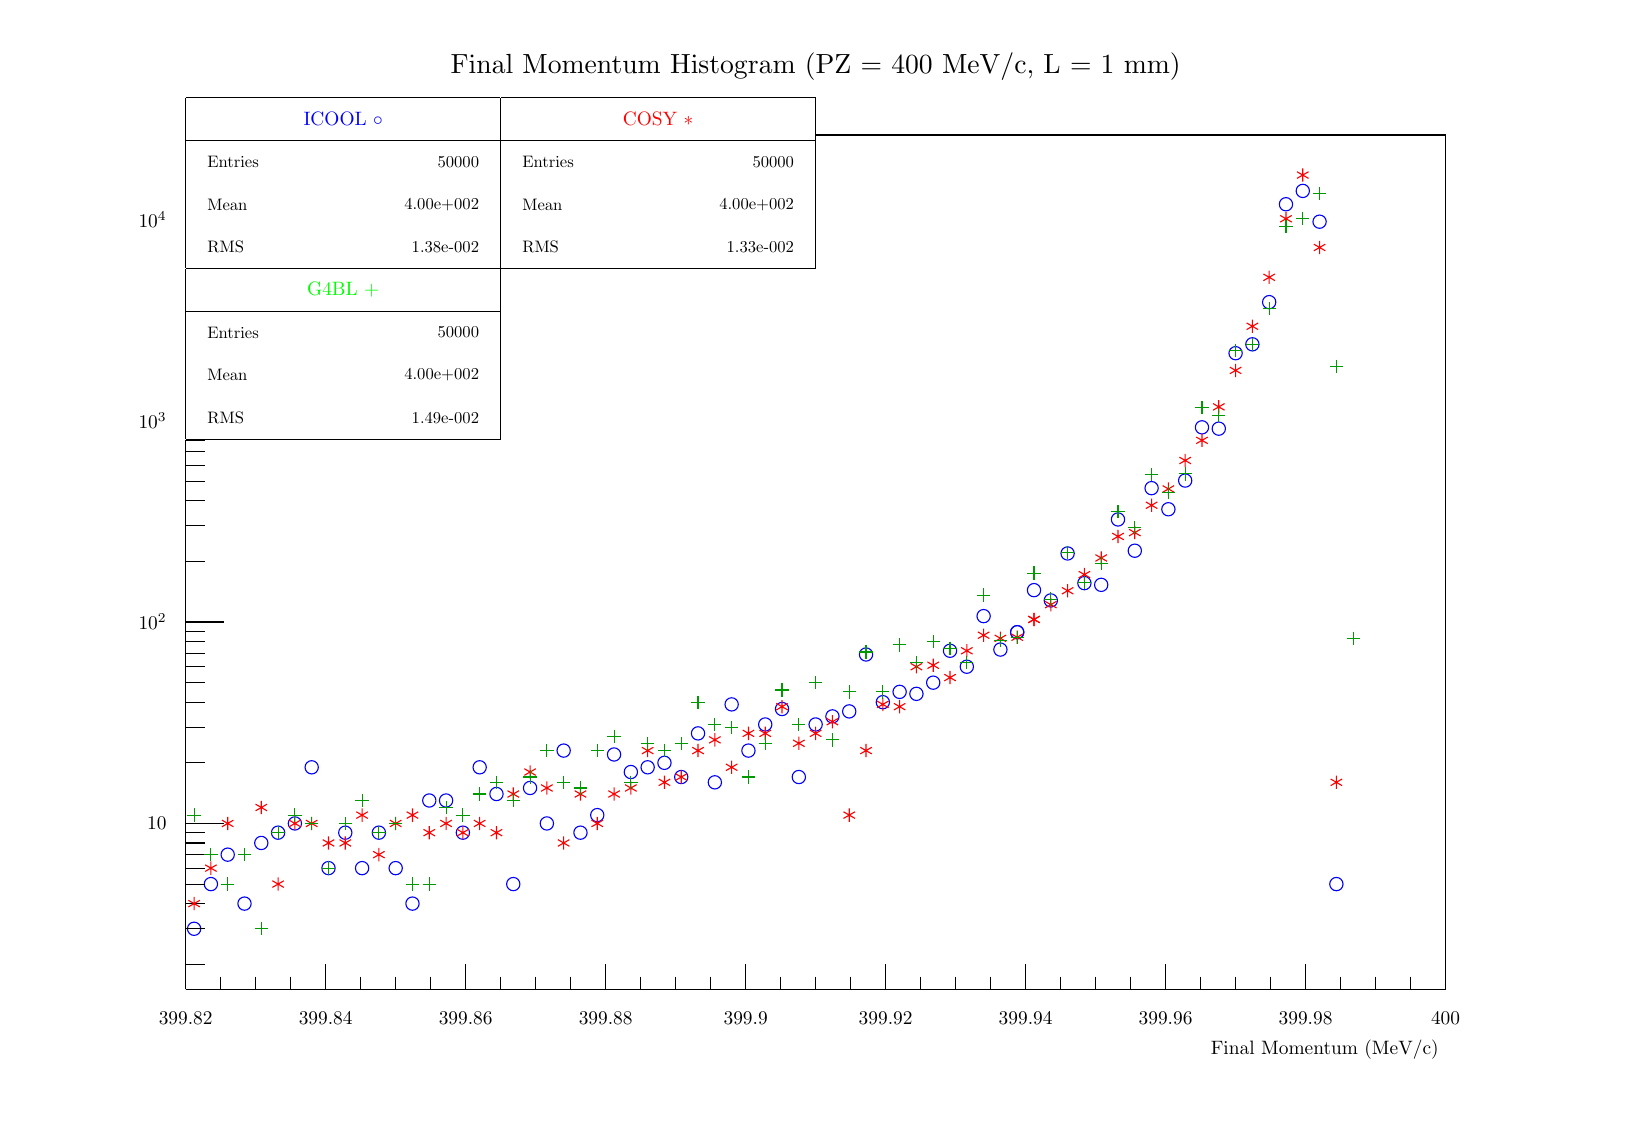
\begin{tikzpicture}
\definecolor{c}{rgb}{1,1,1};
\draw [color=c, fill=c] (0,0) rectangle (20,13.5632);
\draw [color=c, fill=c] (2,1.35632) rectangle (18,12.2069);
\definecolor{c}{rgb}{0,0,0};
\draw [c] (2,1.35632) -- (2,12.2069) -- (18,12.2069) -- (18,1.35632) -- (2,1.35632);
\definecolor{c}{rgb}{1,1,1};
\draw [color=c, fill=c] (2,1.35632) rectangle (18,12.2069);
\definecolor{c}{rgb}{0,0,0};
\draw [c] (2,1.35632) -- (2,12.2069) -- (18,12.2069) -- (18,1.35632) -- (2,1.35632);
\definecolor{c}{rgb}{0,0,1};
\foreach \P in
 {(2.10667,2.12635),(2.32,2.69383),(2.53333,3.06762),(2.74667,2.44594),(2.96,3.21596),(3.17333,3.34681),(3.38667,3.46385),(3.6,4.1769),(3.81333,2.89637),(4.02667,3.34681),(4.24,2.89637),(4.45333,3.34681),(4.66667,2.89637),(4.88,2.44594),(5.09333,3.75
532),(5.30667,3.75532),(5.52,3.34681),(5.73333,4.1769),(5.94667,3.83765),(6.16,2.69383),(6.37333,3.91429),(6.58667,3.46385),(6.8,4.38914),(7.01333,3.34681),(7.22667,3.56974),(7.44,4.33976),(7.65333,4.11683),(7.86667,4.1769),(8.08,4.23388),(8.29333,4.
05334),(8.50667,4.60767),(8.72,3.98599),(8.93333,4.97578),(9.14667,4.38914),(9.36,4.72074),(9.57333,4.9173),(9.78667,4.05334),(10,4.72074),(10.2133,4.82336),(10.4267,4.88686),(10.64,5.6096),(10.8533,5.00391),(11.0667,5.13475),(11.28,5.10979),(11.4933
,5.2518),(11.7067,5.65688),(11.92,5.45434),(12.1333,6.09699),(12.3467,5.67221),(12.56,5.89236)}{\draw[mark options={color=c,fill=c},mark size=2.402402pt,mark=o] plot coordinates {\P};}
\foreach \P in
 {(12.56,5.89236),(12.7733,6.42691),(12.9867,6.29606),(13.2,6.89267),(13.4133,6.51583),(13.6267,6.49426),(13.84,7.32435),(14.0533,6.92762),(14.2667,7.72196),(14.48,7.45405),(14.6933,7.81862),(14.9067,8.49438),(15.12,8.47746),(15.3333,9.43583),(15.546
7,9.54865),(15.76,10.0843),(15.9733,11.3275),(16.1867,11.4969),(16.4,11.1062),(16.6133,2.69383)}{\draw[mark options={color=c,fill=c},mark size=2.402402pt,mark=o] plot coordinates {\P};}
\definecolor{c}{rgb}{1,1,1};
\draw [color=c, fill=c] (2,10.5115) rectangle (6,12.6816);
\definecolor{c}{rgb}{0,0,0};
\draw [c] (2,10.5115) -- (6,10.5115);
\draw [c] (6,10.5115) -- (6,12.6816);
\draw [c] (6,12.6816) -- (2,12.6816);
\draw [c] (2,12.6816) -- (2,10.5115);
\draw[color=blue](4,12.4103) node[scale=0.7, rotate=0]{ICOOL $\circ$};
\draw [c] (2,12.1391) -- (6,12.1391);
\draw [anchor= west] (2.2,11.8678) node[scale=0.6, rotate=0]{Entries };
\draw [anchor= east] (5.8,11.8678) node[scale=0.6, rotate=0]{ 50000};
\draw [anchor= west] (2.2,11.3253) node[scale=0.6, rotate=0]{Mean  };
\draw [anchor= east] (5.8,11.3253) node[scale=0.6, rotate=0]{ 4.00e+002};
\draw [anchor= west] (2.2,10.7828) node[scale=0.6, rotate=0]{RMS   };
\draw [anchor= east] (5.8,10.7828) node[scale=0.6, rotate=0]{ 1.38e-002};
\draw [c] (2,1.35632) -- (18,1.35632);
\draw [anchor= east] (18,0.596782) node[scale=0.7, rotate=0]{Final Momentum (MeV/c)};
\draw [c] (2,1.68184) -- (2,1.35632);
\draw [c] (2.44444,1.51908) -- (2.44444,1.35632);
\draw [c] (2.88889,1.51908) -- (2.88889,1.35632);
\draw [c] (3.33333,1.51908) -- (3.33333,1.35632);
\draw [c] (3.77778,1.68184) -- (3.77778,1.35632);
\draw [c] (4.22222,1.51908) -- (4.22222,1.35632);
\draw [c] (4.66667,1.51908) -- (4.66667,1.35632);
\draw [c] (5.11111,1.51908) -- (5.11111,1.35632);
\draw [c] (5.55556,1.68184) -- (5.55556,1.35632);
\draw [c] (6,1.51908) -- (6,1.35632);
\draw [c] (6.44444,1.51908) -- (6.44444,1.35632);
\draw [c] (6.88889,1.51908) -- (6.88889,1.35632);
\draw [c] (7.33333,1.68184) -- (7.33333,1.35632);
\draw [c] (7.77778,1.51908) -- (7.77778,1.35632);
\draw [c] (8.22222,1.51908) -- (8.22222,1.35632);
\draw [c] (8.66667,1.51908) -- (8.66667,1.35632);
\draw [c] (9.11111,1.68184) -- (9.11111,1.35632);
\draw [c] (9.55556,1.51908) -- (9.55556,1.35632);
\draw [c] (10,1.51908) -- (10,1.35632);
\draw [c] (10.4444,1.51908) -- (10.4444,1.35632);
\draw [c] (10.8889,1.68184) -- (10.8889,1.35632);
\draw [c] (11.3333,1.51908) -- (11.3333,1.35632);
\draw [c] (11.7778,1.51908) -- (11.7778,1.35632);
\draw [c] (12.2222,1.51908) -- (12.2222,1.35632);
\draw [c] (12.6667,1.68184) -- (12.6667,1.35632);
\draw [c] (13.1111,1.51908) -- (13.1111,1.35632);
\draw [c] (13.5556,1.51908) -- (13.5556,1.35632);
\draw [c] (14,1.51908) -- (14,1.35632);
\draw [c] (14.4444,1.68184) -- (14.4444,1.35632);
\draw [c] (14.8889,1.51908) -- (14.8889,1.35632);
\draw [c] (15.3333,1.51908) -- (15.3333,1.35632);
\draw [c] (15.7778,1.51908) -- (15.7778,1.35632);
\draw [c] (16.2222,1.68184) -- (16.2222,1.35632);
\draw [c] (16.6667,1.51908) -- (16.6667,1.35632);
\draw [c] (17.1111,1.51908) -- (17.1111,1.35632);
\draw [c] (17.5556,1.51908) -- (17.5556,1.35632);
\draw [c] (18,1.68184) -- (18,1.35632);
\draw [anchor=base] (2,0.908736) node[scale=0.7, rotate=0]{399.82};
\draw [anchor=base] (3.77778,0.908736) node[scale=0.7, rotate=0]{399.84};
\draw [anchor=base] (5.55556,0.908736) node[scale=0.7, rotate=0]{399.86};
\draw [anchor=base] (7.33333,0.908736) node[scale=0.7, rotate=0]{399.88};
\draw [anchor=base] (9.11111,0.908736) node[scale=0.7, rotate=0]{399.9};
\draw [anchor=base] (10.8889,0.908736) node[scale=0.7, rotate=0]{399.92};
\draw [anchor=base] (12.6667,0.908736) node[scale=0.7, rotate=0]{399.94};
\draw [anchor=base] (14.4444,0.908736) node[scale=0.7, rotate=0]{399.96};
\draw [anchor=base] (16.2222,0.908736) node[scale=0.7, rotate=0]{399.98};
\draw [anchor=base] (18,0.908736) node[scale=0.7, rotate=0]{400};
\draw [c] (2,1.35632) -- (2,12.2069);
\draw [c] (2.24,1.67591) -- (2,1.67591);
\draw [c] (2.24,2.12634) -- (2,2.12634);
\draw [c] (2.24,2.44593) -- (2,2.44593);
\draw [c] (2.24,2.69383) -- (2,2.69383);
\draw [c] (2.24,2.89637) -- (2,2.89637);
\draw [c] (2.24,3.06762) -- (2,3.06762);
\draw [c] (2.24,3.21596) -- (2,3.21596);
\draw [c] (2.24,3.34681) -- (2,3.34681);
\draw [c] (2.48,3.46385) -- (2,3.46385);
\draw [anchor= east] (1.844,3.46385) node[scale=0.7, rotate=0]{10};
\draw [c] (2.24,4.23388) -- (2,4.23388);
\draw [c] (2.24,4.68431) -- (2,4.68431);
\draw [c] (2.24,5.0039) -- (2,5.0039);
\draw [c] (2.24,5.2518) -- (2,5.2518);
\draw [c] (2.24,5.45434) -- (2,5.45434);
\draw [c] (2.24,5.62559) -- (2,5.62559);
\draw [c] (2.24,5.77393) -- (2,5.77393);
\draw [c] (2.24,5.90478) -- (2,5.90478);
\draw [c] (2.48,6.02182) -- (2,6.02182);
\draw [anchor= east] (1.844,6.02182) node[scale=0.7, rotate=0]{$10^{2}$};
\draw [c] (2.24,6.79185) -- (2,6.79185);
\draw [c] (2.24,7.24228) -- (2,7.24228);
\draw [c] (2.24,7.56187) -- (2,7.56187);
\draw [c] (2.24,7.80977) -- (2,7.80977);
\draw [c] (2.24,8.01231) -- (2,8.01231);
\draw [c] (2.24,8.18356) -- (2,8.18356);
\draw [c] (2.24,8.3319) -- (2,8.3319);
\draw [c] (2.24,8.46274) -- (2,8.46274);
\draw [c] (2.48,8.57979) -- (2,8.57979);
\draw [anchor= east] (1.844,8.57979) node[scale=0.7, rotate=0]{$10^{3}$};
\draw [c] (2.24,9.34982) -- (2,9.34982);
\draw [c] (2.24,9.80025) -- (2,9.80025);
\draw [c] (2.24,10.1198) -- (2,10.1198);
\draw [c] (2.24,10.3677) -- (2,10.3677);
\draw [c] (2.24,10.5703) -- (2,10.5703);
\draw [c] (2.24,10.7415) -- (2,10.7415);
\draw [c] (2.24,10.8899) -- (2,10.8899);
\draw [c] (2.24,11.0207) -- (2,11.0207);
\draw [c] (2.48,11.1378) -- (2,11.1378);
\draw [anchor= east] (1.844,11.1378) node[scale=0.7, rotate=0]{$10^{4}$};
\draw [c] (2.24,11.9078) -- (2,11.9078);
\definecolor{c}{rgb}{1,1,1};
\draw [color=c, fill=c] (2,10.5115) rectangle (6,12.6816);
\definecolor{c}{rgb}{0,0,0};
\draw [c] (2,10.5115) -- (6,10.5115);
\draw [c] (6,10.5115) -- (6,12.6816);
\draw [c] (6,12.6816) -- (2,12.6816);
\draw [c] (2,12.6816) -- (2,10.5115);
\draw[color=blue](4,12.4103) node[scale=0.7, rotate=0]{ICOOL $\circ$};
\draw [c] (2,12.1391) -- (6,12.1391);
\draw [anchor= west] (2.2,11.8678) node[scale=0.6, rotate=0]{Entries };
\draw [anchor= east] (5.8,11.8678) node[scale=0.6, rotate=0]{ 50000};
\draw [anchor= west] (2.2,11.3253) node[scale=0.6, rotate=0]{Mean  };
\draw [anchor= east] (5.8,11.3253) node[scale=0.6, rotate=0]{ 4.00e+002};
\draw [anchor= west] (2.2,10.7828) node[scale=0.6, rotate=0]{RMS   };
\draw [anchor= east] (5.8,10.7828) node[scale=0.6, rotate=0]{ 1.38e-002};
\draw (10,13.0816) node[scale=1, rotate=0]{Final Momentum Histogram (PZ = 400 MeV/c, L = 1 mm)};
\definecolor{c}{rgb}{1,0,0};
\foreach \P in
 {(2.10667,2.44594),(2.32,2.89637),(2.53333,3.46385),(2.96,3.6664),(3.17333,2.69383),(3.38667,3.46385),(3.6,3.46385),(3.81333,3.21596),(4.02667,3.21596),(4.24,3.56974),(4.45333,3.06762),(4.66667,3.46385),(4.88,3.56974),(5.09333,3.34681),(5.30667,3.46
385),(5.52,3.34681),(5.73333,3.46385),(5.94667,3.34681),(6.16,3.83765),(6.37333,4.11683),(6.58667,3.91429),(6.8,3.21596),(7.01333,3.83765),(7.22667,3.46385),(7.44,3.83765),(7.65333,3.91429),(7.86667,4.38914),(8.08,3.98599),(8.29333,4.05334),(8.50667,
4.38914),(8.72,4.52534),(8.93333,4.1769),(9.14667,4.60767),(9.36,4.60767),(9.57333,4.94692),(9.78667,4.48177),(10,4.60767),(10.2133,4.75601),(10.4267,3.56974),(10.64,4.38914),(10.8533,4.97578),(11.0667,4.94692),(11.28,5.45434),(11.4933,5.4727),(11.70
67,5.31653),(11.92,5.65688),(12.1333,5.85427),(12.3467,5.81483),(12.56,5.82813),(12.7733,6.05466)}{\draw[mark options={color=c,fill=c},mark size=2.402402pt,mark=asterisk] plot coordinates {\P};}
\foreach \P in
 {(12.7733,6.05466),(12.9867,6.24273),(13.2,6.41917),(13.4133,6.6243),(13.6267,6.83542),(13.84,7.10866),(14.0533,7.15768),(14.2667,7.50489),(14.48,7.7123),(14.6933,8.07354),(14.9067,8.32912),(15.12,8.75421),(15.3333,9.21723),(15.5467,9.77781),(15.76,
10.3997),(15.9733,11.1433),(16.1867,11.6984),(16.4,10.7784),(16.6133,3.98599)}{\draw[mark options={color=c,fill=c},mark size=2.402402pt,mark=asterisk] plot coordinates {\P};}
\definecolor{c}{rgb}{1,1,1};
\draw [color=c, fill=c] (6,10.5115) rectangle (10,12.6816);
\definecolor{c}{rgb}{0,0,0};
\draw [c] (6,10.5115) -- (10,10.5115);
\draw [c] (10,10.5115) -- (10,12.6816);
\draw [c] (10,12.6816) -- (6,12.6816);
\draw [c] (6,12.6816) -- (6,10.5115);
\draw [color=red](8,12.4103) node[scale=0.7, rotate=0]{COSY $*$};
\draw [c] (6,12.1391) -- (10,12.1391);
\draw [anchor= west] (6.2,11.8678) node[scale=0.6, rotate=0]{Entries };
\draw [anchor= east] (9.8,11.8678) node[scale=0.6, rotate=0]{ 50000};
\draw [anchor= west] (6.2,11.3253) node[scale=0.6, rotate=0]{Mean  };
\draw [anchor= east] (9.8,11.3253) node[scale=0.6, rotate=0]{ 4.00e+002};
\draw [anchor= west] (6.2,10.7828) node[scale=0.6, rotate=0]{RMS   };
\draw [anchor= east] (9.8,10.7828) node[scale=0.6, rotate=0]{ 1.33e-002};
\definecolor{c}{rgb}{1,1,1};
\draw [color=c, fill=c] (6,10.5115) rectangle (10,12.6816);
\definecolor{c}{rgb}{0,0,0};
\draw [c] (6,10.5115) -- (10,10.5115);
\draw [c] (10,10.5115) -- (10,12.6816);
\draw [c] (10,12.6816) -- (6,12.6816);
\draw [c] (6,12.6816) -- (6,10.5115);
\draw [color=red](8,12.4103) node[scale=0.7, rotate=0]{COSY $*$};
\draw [c] (6,12.1391) -- (10,12.1391);
\draw [anchor= west] (6.2,11.8678) node[scale=0.6, rotate=0]{Entries };
\draw [anchor= east] (9.8,11.8678) node[scale=0.6, rotate=0]{ 50000};
\draw [anchor= west] (6.2,11.3253) node[scale=0.6, rotate=0]{Mean  };
\draw [anchor= east] (9.8,11.3253) node[scale=0.6, rotate=0]{ 4.00e+002};
\draw [anchor= west] (6.2,10.7828) node[scale=0.6, rotate=0]{RMS   };
\draw [anchor= east] (9.8,10.7828) node[scale=0.6, rotate=0]{ 1.33e-002};
\definecolor{c}{rgb}{0,0.6,0};
\foreach \P in
 {(2.10667,3.56974),(2.32,3.06762),(2.53333,2.69383),(2.74667,3.06762),(2.96,2.12635),(3.17333,3.34681),(3.38667,3.56974),(3.6,3.46385),(3.81333,2.89637),(4.02667,3.46385),(4.24,3.75532),(4.45333,3.34681),(4.66667,3.46385),(4.88,2.69383),(5.09333,2.6
9383),(5.30667,3.6664),(5.52,3.56974),(5.73333,3.83765),(5.94667,3.98599),(6.16,3.75532),(6.37333,4.05334),(6.58667,4.38914),(6.8,3.98599),(7.01333,3.91429),(7.22667,4.38914),(7.44,4.56727),(7.65333,3.98599),(7.86667,4.48177),(8.08,4.38914),(8.29333,
4.48177),(8.50667,5.00391),(8.72,4.72074),(8.93333,4.68432),(9.14667,4.05334),(9.36,4.48177),(9.57333,5.15917),(9.78667,4.72074),(10,5.2518),(10.2133,4.52534),(10.4267,5.13475),(10.64,5.64135),(10.8533,5.13475),(11.0667,5.73147),(11.28,5.50854),(11.4
933,5.77393),(11.7067,5.68732),(11.92,5.50854),(12.1333,6.36341),(12.3467,5.78773),(12.56,5.82813)}{\draw[mark options={color=c,fill=c},mark size=2.402402pt,mark=+] plot coordinates {\P};}
\foreach \P in
 {(12.56,5.82813),(12.7733,6.64351),(12.9867,6.31329),(13.2,6.90778),(13.4133,6.52293),(13.6267,6.76941),(13.84,7.42616),(14.0533,7.21984),(14.2667,7.89114),(14.48,7.66776),(14.6933,7.90346),(14.9067,8.74563),(15.12,8.64557),(15.3333,9.47224),(15.546
7,9.54493),(15.76,10.0031),(15.9733,11.043),(16.1867,11.1496),(16.4,11.4623),(16.6133,9.26621),(16.8267,5.81483)}{\draw[mark options={color=c,fill=c},mark size=2.402402pt,mark=+] plot coordinates {\P};}
\definecolor{c}{rgb}{1,1,1};
\draw [color=c, fill=c] (2,8.34138) rectangle (6,10.5115);
\definecolor{c}{rgb}{0,0,0};
\draw [c] (2,8.34138) -- (6,8.34138);
\draw [c] (6,8.34138) -- (6,10.5115);
\draw [c] (6,10.5115) -- (2,10.5115);
\draw [c] (2,10.5115) -- (2,8.34138);
\draw [color=green](4,10.2402) node[scale=0.7, rotate=0]{G4BL $+$};
\draw [c] (2,9.96897) -- (6,9.96897);
\draw [anchor= west] (2.2,9.6977) node[scale=0.6, rotate=0]{Entries };
\draw [anchor= east] (5.8,9.6977) node[scale=0.6, rotate=0]{ 50000};
\draw [anchor= west] (2.2,9.15517) node[scale=0.6, rotate=0]{Mean  };
\draw [anchor= east] (5.8,9.15517) node[scale=0.6, rotate=0]{ 4.00e+002};
\draw [anchor= west] (2.2,8.61264) node[scale=0.6, rotate=0]{RMS   };
\draw [anchor= east] (5.8,8.61264) node[scale=0.6, rotate=0]{ 1.49e-002};
\definecolor{c}{rgb}{1,1,1};
\draw [color=c, fill=c] (2,8.34138) rectangle (6,10.5115);
\definecolor{c}{rgb}{0,0,0};
\draw [c] (2,8.34138) -- (6,8.34138);
\draw [c] (6,8.34138) -- (6,10.5115);
\draw [c] (6,10.5115) -- (2,10.5115);
\draw [c] (2,10.5115) -- (2,8.34138);
\draw [color=green](4,10.2402) node[scale=0.7, rotate=0]{G4BL $+$};
\draw [c] (2,9.96897) -- (6,9.96897);
\draw [anchor= west] (2.2,9.6977) node[scale=0.6, rotate=0]{Entries };
\draw [anchor= east] (5.8,9.6977) node[scale=0.6, rotate=0]{ 50000};
\draw [anchor= west] (2.2,9.15517) node[scale=0.6, rotate=0]{Mean  };
\draw [anchor= east] (5.8,9.15517) node[scale=0.6, rotate=0]{ 4.00e+002};
\draw [anchor= west] (2.2,8.61264) node[scale=0.6, rotate=0]{RMS   };
\draw [anchor= east] (5.8,8.61264) node[scale=0.6, rotate=0]{ 1.49e-002};
\end{tikzpicture}
